\documentclass[a4paper, 10pt]{article}
\usepackage[UTF8]{ctex}
\usepackage{subfigure}
\usepackage[graphicx]{realboxes}
\begin{document}
  \title{实验报告:迈克尔逊干涉仪}
  \author{郑志恒 2300012559}
  \maketitle
\section{实验装置}
\begin{figure}[h]
    \centering %表示居中
    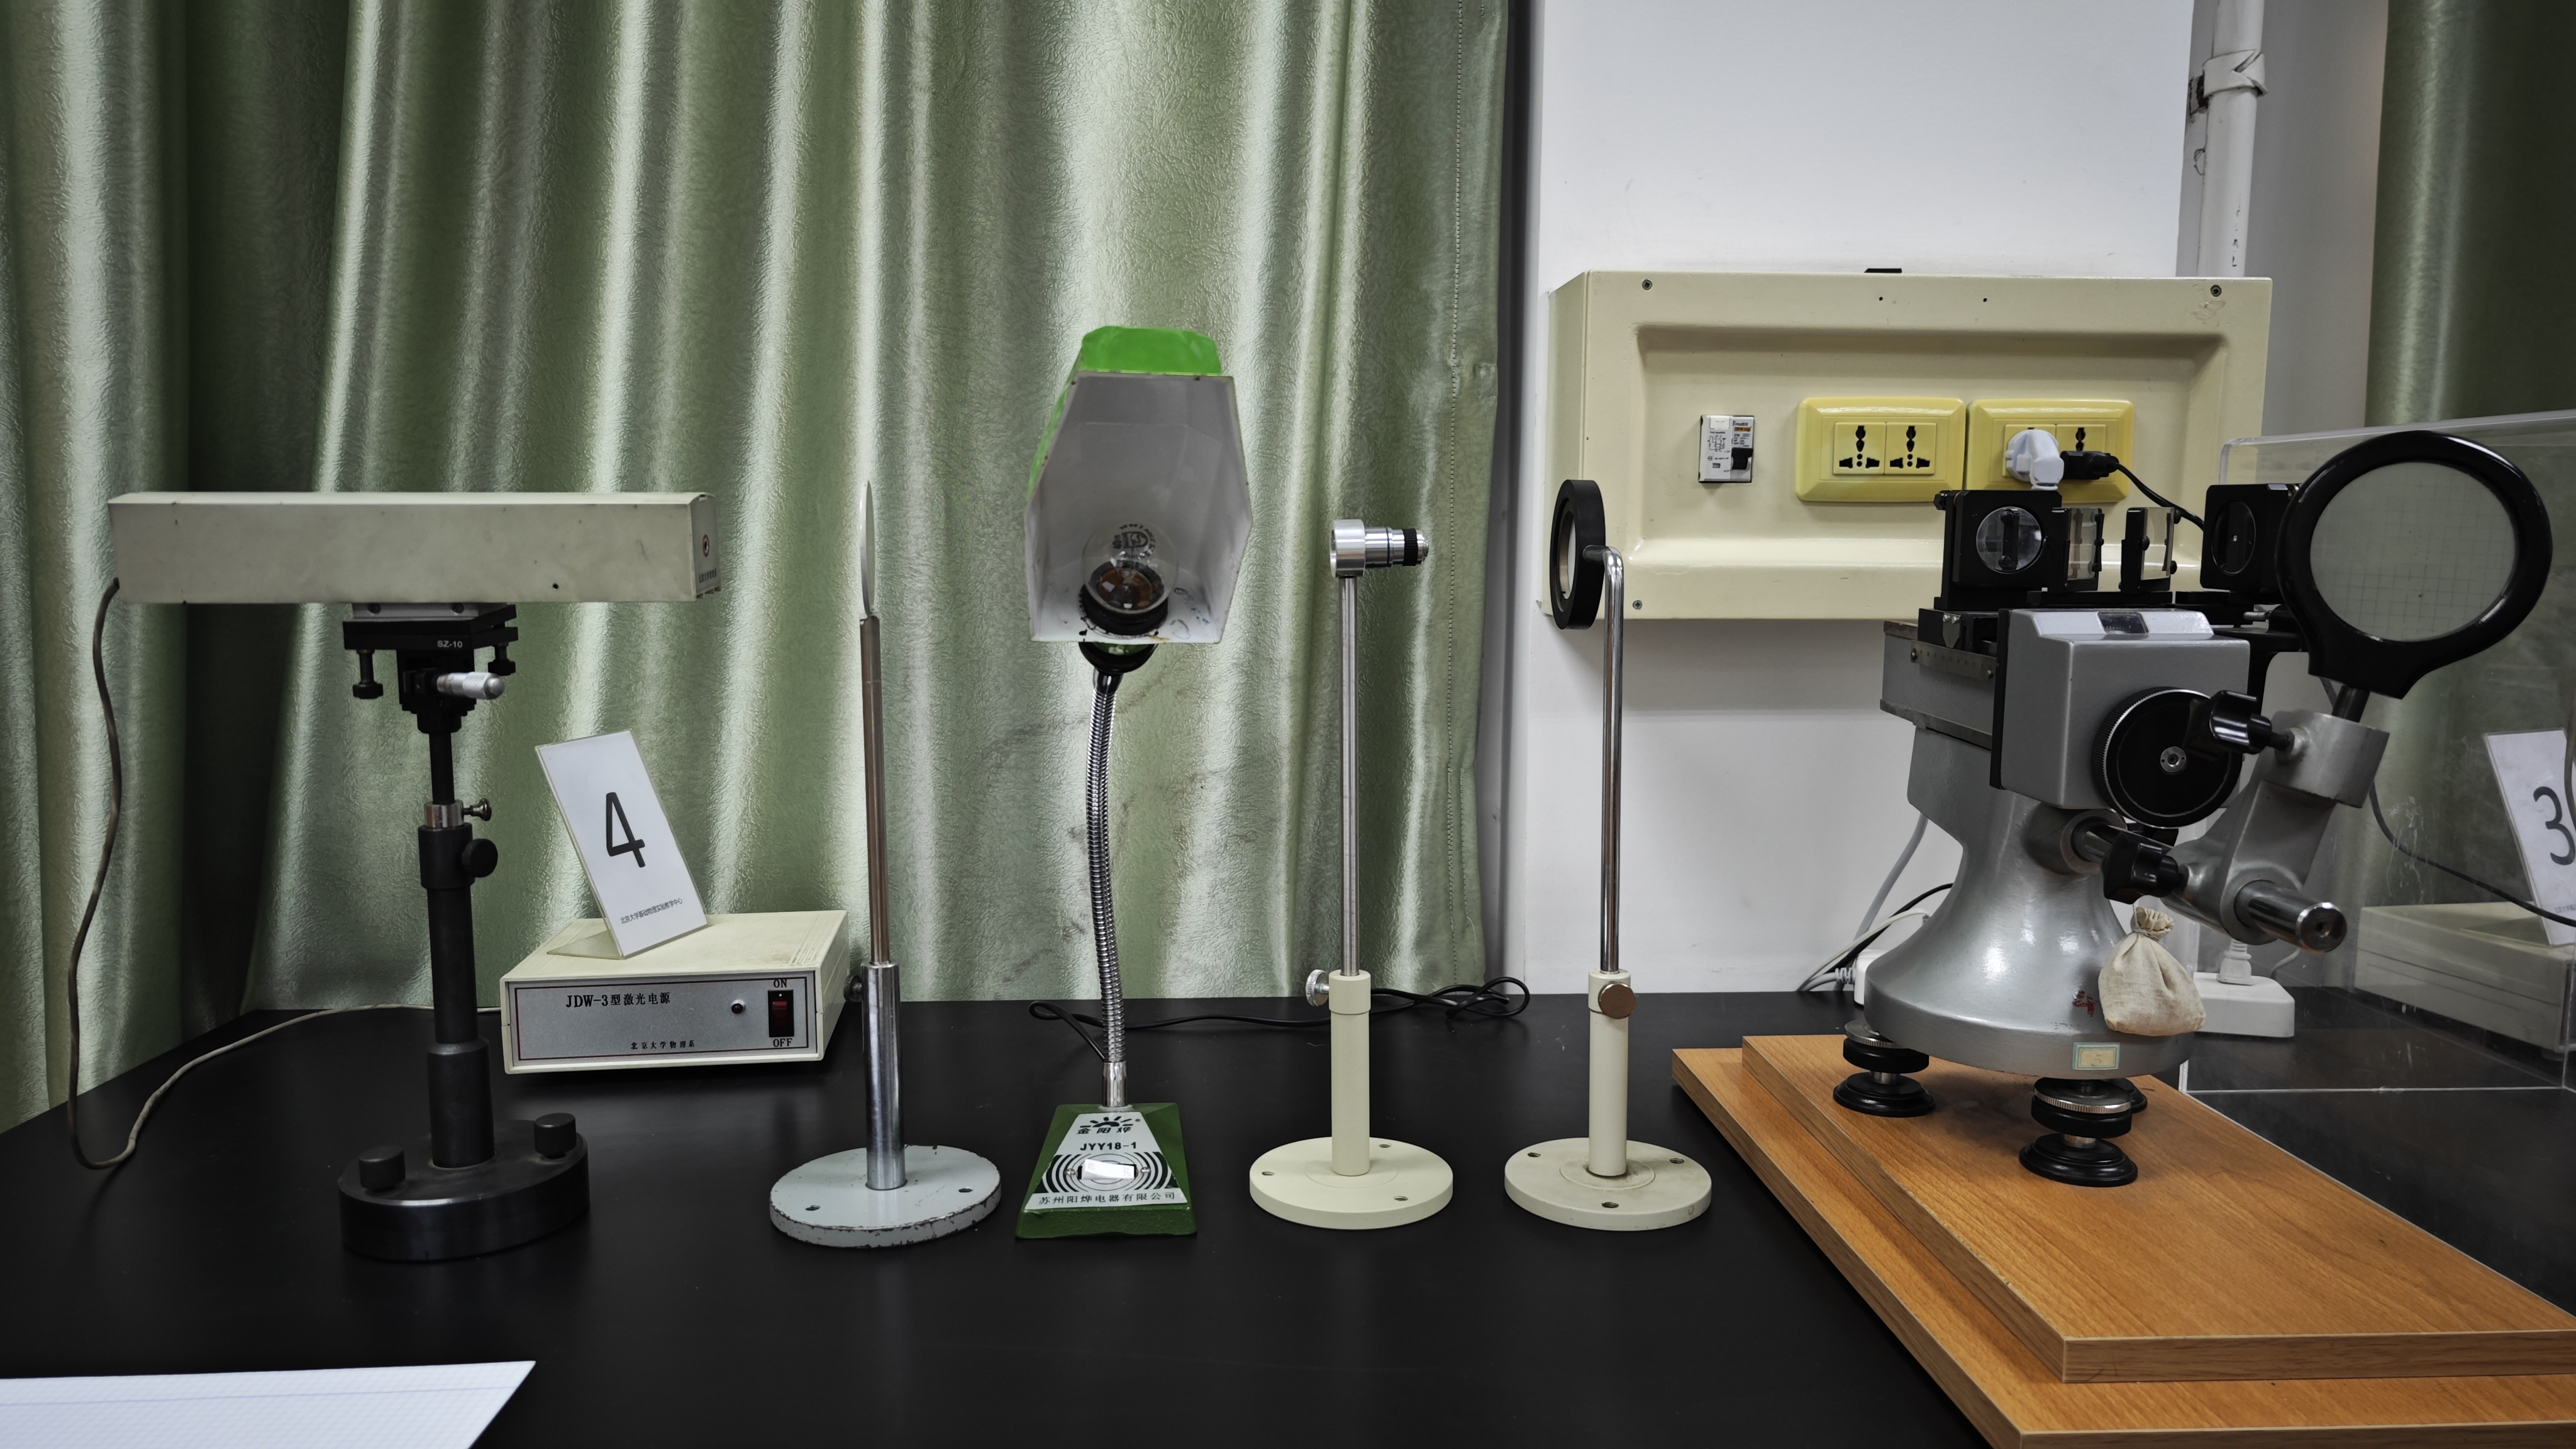
\includegraphics[height=4.5cm,width=9.5cm]{p1.jpg}
    
    \caption{实验装置图}
    
    \label{2}
    
\end{figure}
\noindent 从左到右依次为:激光器、小孔、白光灯、短焦凸透镜、毛玻璃、Michelson干涉仪

\section{Michelson干涉仪的调节步骤}
\noindent 1.将Michelson干涉仪调节完毕使得光屏上已经能看到干涉条纹。调节激光器水平:打开激光器,调节激光器的角度和高度,使激光刚好能穿过小孔;改变小孔与激光器的距离,并重新调节激光器的高度和角度,使得无论小孔与激光器的距离为多少,激光始终能穿过小孔。

\noindent 2.将激光器通过小孔对准Michelson干涉仪的分束镜G1,以45度角入射,此时可以看到小孔面上出现两组光斑,两组光斑分别对应M1和M2的反射,通过调节M1和M2背后的螺丝调整M1和M2的角度,使得每组光斑的中心光斑都与小孔重合。

\noindent 3.将短焦透镜对准激光束,调节透镜的高度使得激光束刚好通过短焦透镜,制造点光源。此时激光束通过短焦透镜以45度入射分束镜,可以在光屏上看到干涉条纹,说明Michelson干涉仪已经调节完毕。
\section{各种干涉条纹图样的调节和解释}
\subsection{非定域干涉-圆条纹}
\noindent 1.调节M1和M2的纵向距离(z方向),使得M1和M2的z方向距离变大,直到能看到圆条纹的中心。

\begin{figure}[h]
  \centering 
  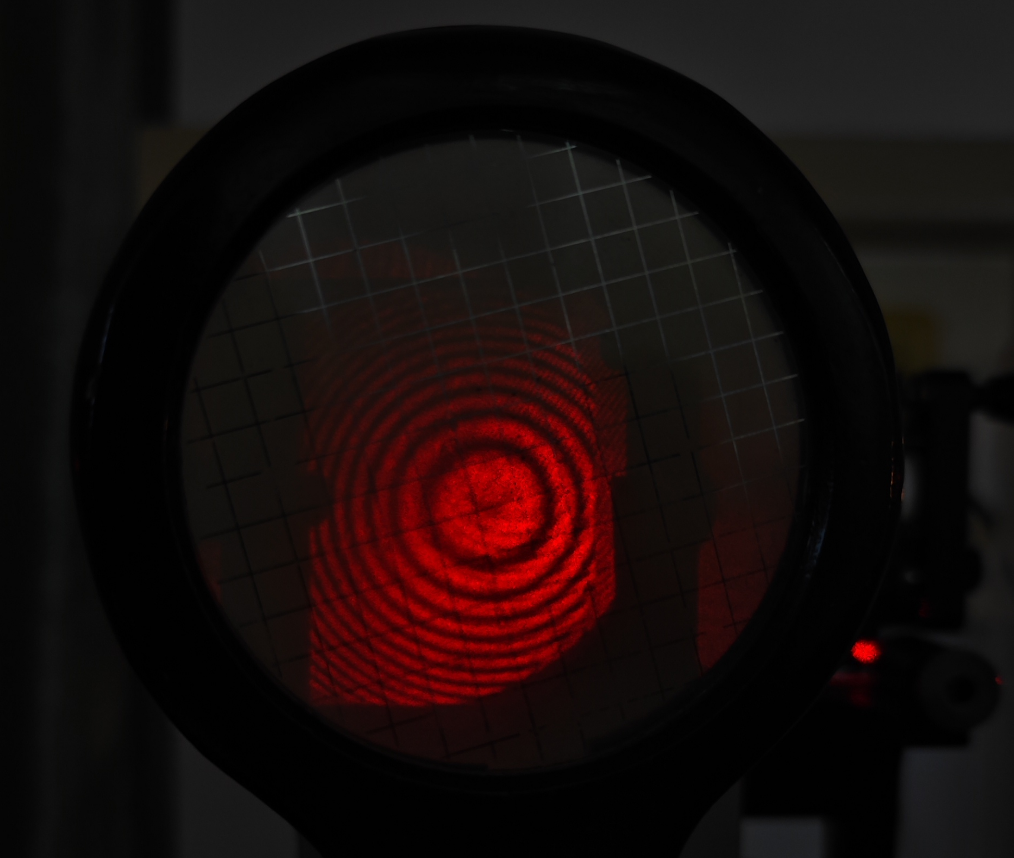
\includegraphics[height=5.0cm,width=6.0cm]{p2.png}
  
  \caption{细圆条纹}
  \label{3}
  
  \end{figure}
  
\noindent 2.微调M2背后控制x和y方向的螺丝,使得圆条纹的中心处于光屏中心。


\noindent 3.调节M1和M2的纵向距离(z方向),使得M1和M2的z方向距离变小,这一过程中能看到光屏上不断“吞”条纹,条纹宽度不断增大。


\noindent 4.重复步骤2和3,保持圆条纹中心一直处于光屏中心的同时不断“吞掉”条纹,即使得M1和M2的纵向距离不断靠近,直到光屏中出现比较粗的圆条纹。
\begin{figure}[h]
  \centering 
  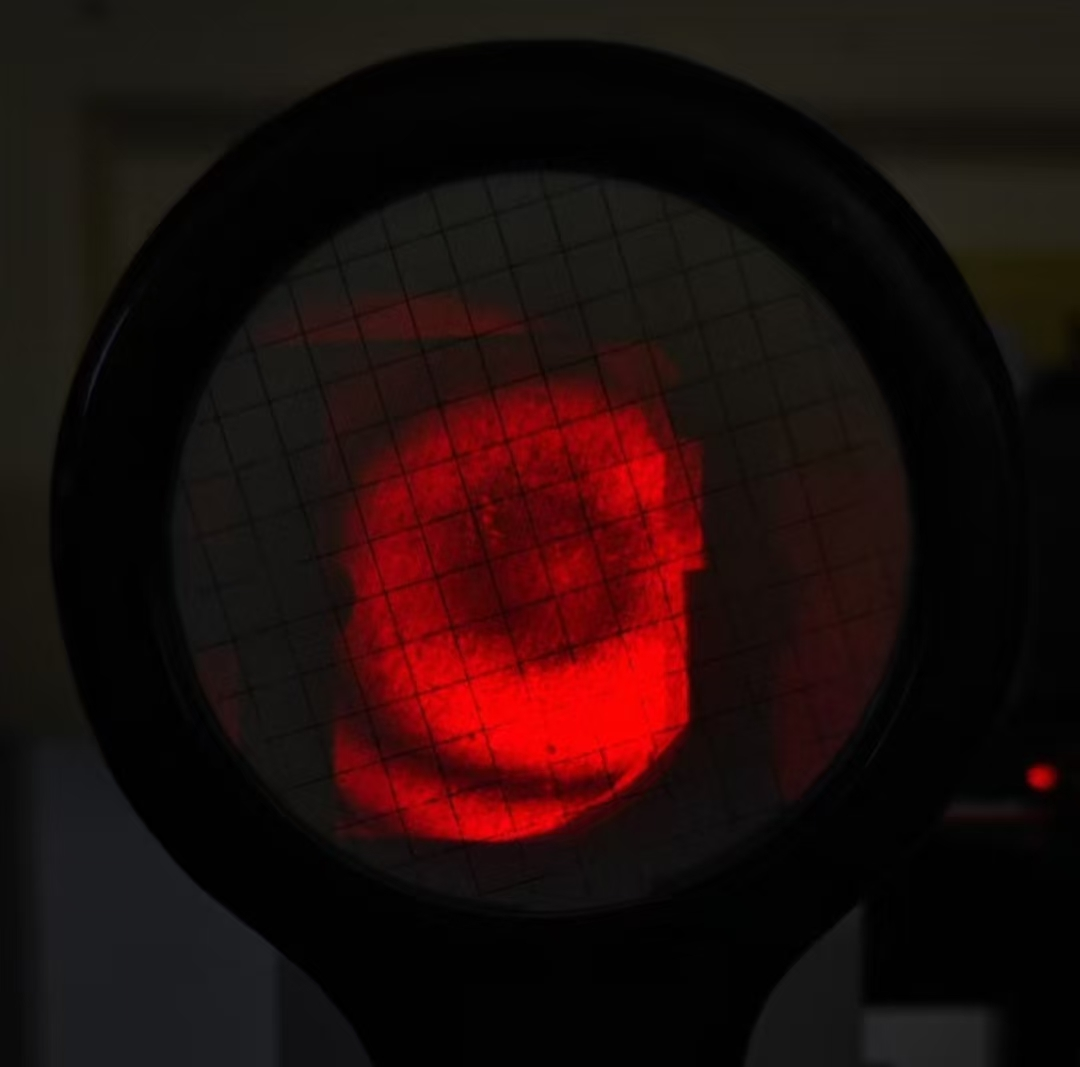
\includegraphics[height=5.0cm,width=5.0cm]{p3.jpg}
  
  \caption{粗圆条纹}
  \label{4}
  
  \end{figure}


\noindent 变化规律与解释:


\noindent 出现圆条纹的条件是两个“像点”的连线平行于z轴,即两个像点没有x和y方向的距离。因此,调节圆条纹的中心位置处于光屏中心的过程使得两个像点没有x和y方向距离,调节纵向距离的过程使得两束光的光程差减小,条纹宽度不断增大。

\noindent 光程差为:
$$\Delta L=2d(1-\frac{r^2}{2z^2})$$
由亮纹条件:
$$\Delta L=k\lambda$$
可以得到条纹间距:
$$\Delta x=\frac{\lambda z^2}{2r_kd}$$
\subsection{非定域干涉-直条纹}
\noindent 1.先经过前面的步骤,调出粗圆条纹。

\noindent 2.调节M2后面的螺钉,使M1和M2出现一个小角度。

\noindent 3.调节M1和M2的纵向距离(z方向),可以看到直条纹。
\begin{figure}[h]
  \centering 
  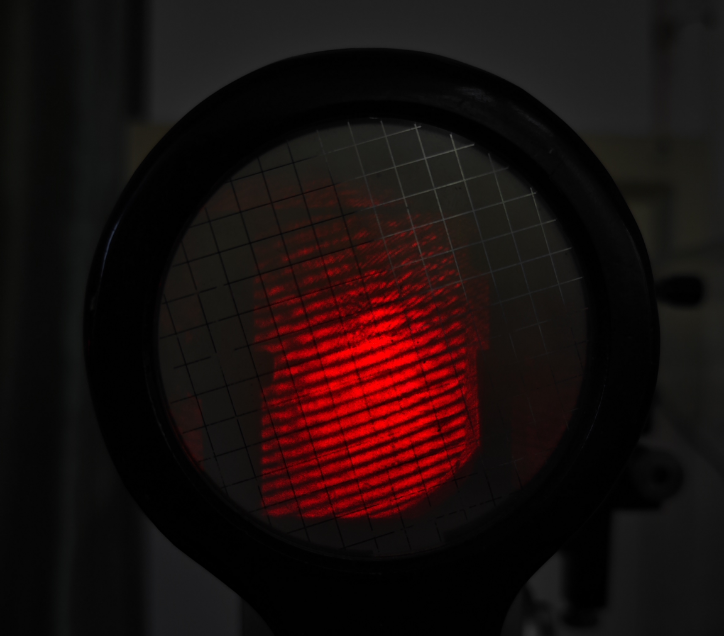
\includegraphics[height=5.0cm,width=5.5cm]{p4.png}
  
  \caption{直条纹}
  \label{5}
  
  \end{figure}


\noindent 变化规律与解释:

\noindent 出现直条纹的条件是两个“像点”的垂直平分线与z轴平行。粗圆条纹时,两个像点基本没有z轴方向的距离。此时调整M2出现一个小角度,即可使得两个像点在横向错开一个距离。此时再微调z轴距离,使得两个像点的垂直平分线平行于z轴,即可在光屏上观察到直条纹。

\subsection{定域干涉-圆条纹}
\noindent 1.经过前面叙述的步骤,先调出条纹中心在光屏中心的圆条纹。

\noindent 2.将毛玻璃放在短焦透镜和Michelson干涉仪之间(为了提高亮度,应当尽量使短焦透镜和毛玻璃之间的距离较大)。此时光屏上的干涉条纹消失。

\noindent 3.将光屏撤下,用眼睛观察,可以看到圆条纹成像。


\begin{figure}[h]
  \centering 
  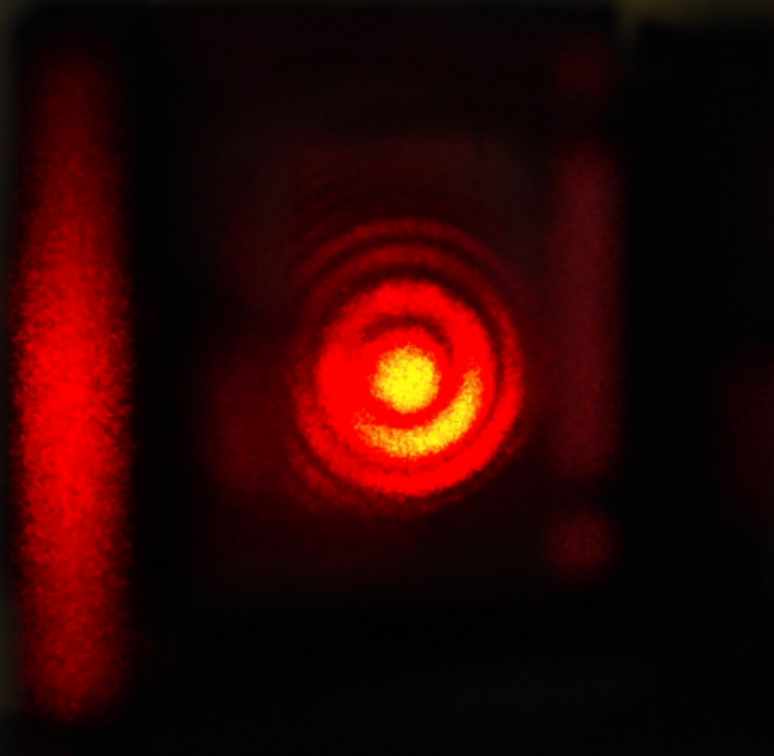
\includegraphics[height=5.0cm,width=5.5cm]{p5.png}
  
  \caption{圆条纹}
  \label{6}

\end{figure}

\noindent 变化规律与解释:

\noindent 此时的干涉相等于等倾干涉,由眼睛作为透镜来聚焦不同角度的光线,可以看到圆条纹成像在无穷远,干涉条纹中间稀疏,边缘密集。
圆心处有:
$$\Delta L=n\lambda=2d$$
对k级条纹有:
$$k\lambda=2dcos\theta_k$$
条纹间距有:
$$\Delta \theta_k=\frac{\lambda}{2k\theta_k}$$

\subsection{定域干涉-直条纹}
\noindent 1.经过前面叙述的步骤,先调出成像在光屏上的非定域干涉直条纹。

\noindent 2.将毛玻璃放在短焦透镜和Michelson干涉仪之间(为了提高亮度,应当尽量使短焦透镜和毛玻璃之间的距离较大)。此时光屏上的干涉条纹消失。

\noindent 3.将光屏撤下,用眼睛观察,可以看到直条纹成像。

\begin{figure}[h]
  \centering 
  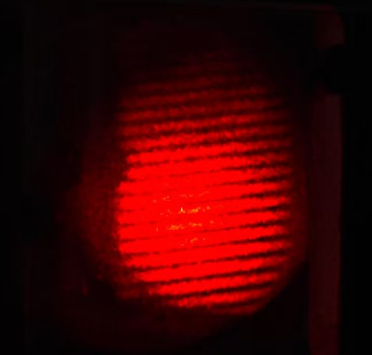
\includegraphics[height=5.0cm,width=5.0cm]{p6.png}
  
  \caption{直条纹}
  \label{7}

\end{figure}

\noindent 变化规律与解释:

\noindent 此时的干涉相当于等厚干涉,由眼睛作为透镜来聚焦不同角度的光线,可以看到直条纹成像在无穷远处。
此时有:
$$\Delta L=2d(1-\frac{\theta^2}{2})$$
有亮纹条件:
$$\Delta L=k\lambda$$
直条纹时,有:
$$\theta=0$$
可以得到条纹间距:
$$\Delta x=\frac{\lambda}{2\alpha}$$
其中$\alpha$是等效薄膜两表面之间的夹角。

\subsection{白光干涉}
\noindent 1.经过前面叙述的步骤,先调出等厚干涉的直条纹。

\noindent 2.打开白光灯,以红条纹为辅助,缓缓调节z轴距离,直到观察到白光的干涉条纹。

\noindent 3.关闭激光器,观察白光干涉条纹,记录z轴距离。

\begin{figure}[h]
  \centering 
  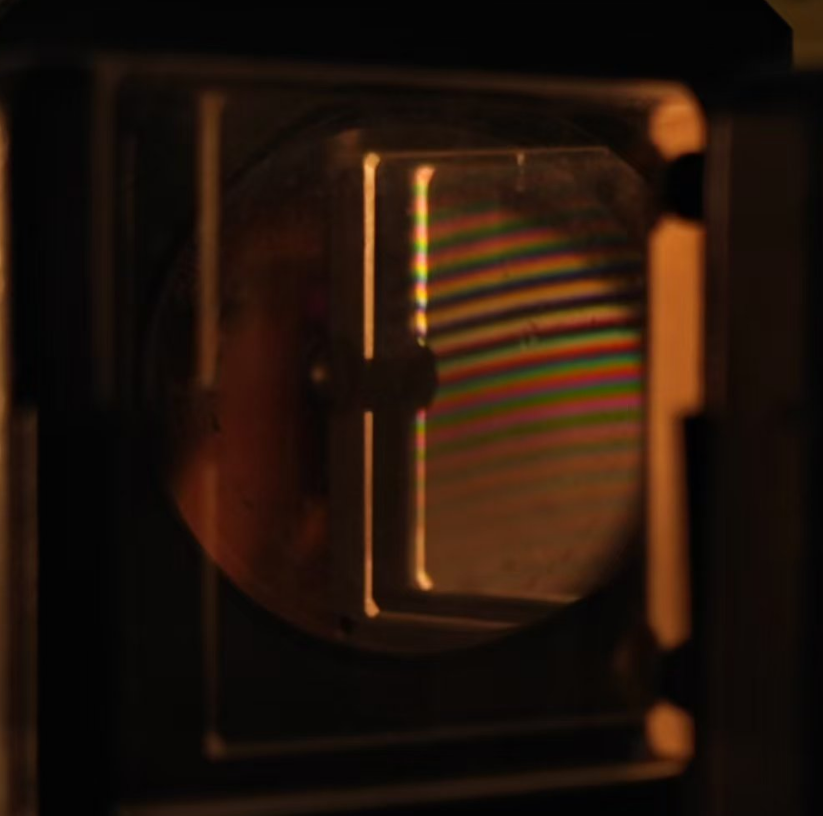
\includegraphics[height=5.0cm,width=5.0cm]{p7.png}
  
  \caption{白光干涉条纹}
  \label{8}

\end{figure}

\noindent 此时记录到z轴距离为$l=51.8mm$.

\noindent 变化规律与解释:

\noindent 此时的干涉也相当于等厚干涉,由眼睛作为透镜来聚焦不同角度的光线,可以看到直条纹成像在无穷远处。
此时有:
$$\Delta L=2d(1-\frac{\theta^2}{2})$$
有亮纹条件:
$$\Delta L=k\lambda$$
直条纹时,有:
$$\theta=0$$
可以得到条纹间距:
$$\Delta x=\frac{\lambda}{2\alpha}$$
其中$\alpha$是等效薄膜两表面之间的夹角。需要注意的是,白光不是单色光,即此时$\lambda$为多值,因此只能观察到中心的少数几条干涉条纹,当距离过大时,不同波长的亮纹和暗纹重合,衬比度下降,观察不到干涉条纹。

\section{激光波长的测量}
\noindent 1.经过前面叙述的步骤,先调出成像在光屏上的非定域干涉圆条纹。

\noindent 2.调节z轴距离,记录中心吞吐的环数n和z轴的调节距离l,并记录数据。

 \begin{tabular}{c|c|c|c|c|c|c}
 0 & 1 & 2 & 3 & 4 & 5 & 6 \\
 n & 10 & 20 & 30 & 40 & 50 & 60  \\
 l($\mu m$) & 3.21 & 6.38 & 9.49 & 12.80 & 15.98 & 19.09 \\
 \end{tabular}
得到拟合的图形为:
\begin{figure}[h]
  \centering 
  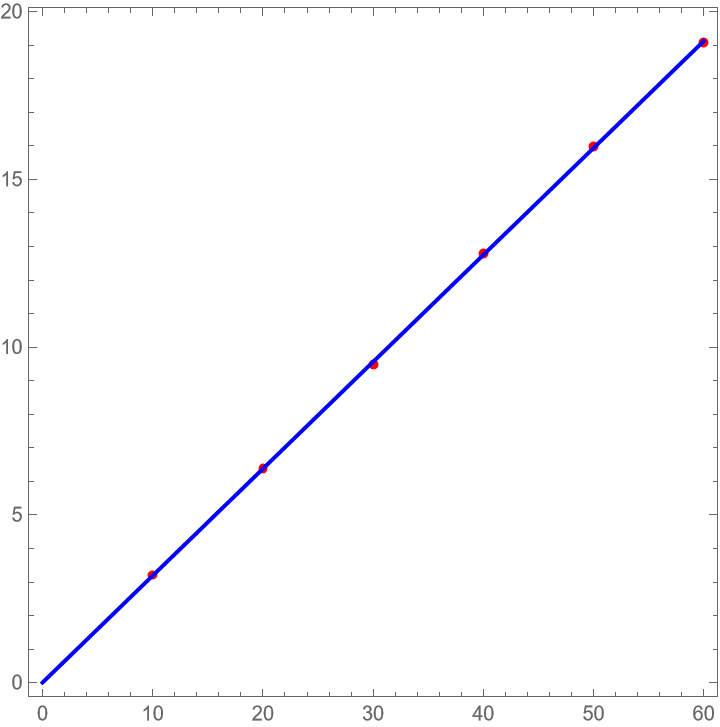
\includegraphics[height=5.0cm,width=5.0cm]{p8.png}
  
  \caption{数据拟合}
  \label{9}

\end{figure}

得到激光的波长大约为:
$$\lambda=\frac{2l}{n}=637.5nm$$

\section{思考题}
\subsection{为什么分束镜的反射与透射光强要求1:1}
\noindent 答:若两束光的振幅相差太大,则干涉条纹的衬比度会相对较低,观察起来不明显。为了使条纹便于观察,要求分束镜的透反比为1:1.
\subsection{为什么眼睛移动时,条纹不吞吐则为严格等倾干涉}
\noindent 答:严格等倾干涉时,光程差只与光线与z轴的夹角有关。当眼睛移动时条纹出现吞吐,说明此时光程差不止与光线和z轴的倾角有关,因此如果眼睛移动时观察到条纹吞吐,则说明此时为非严格等倾干涉,否则为严格等倾干涉。
\subsection{刚开始调准直的时候观察到的多个光点的解释}
\noindent 答:‌迈克尔逊干涉仪调准直时出现的多个光点主要是由于光在分光板的多次反射造成的。其中,中心的亮斑为正常反射得到的光斑,为最亮的光斑。同时,由于两束光经过分光镜时产生了光程差,从而两束光发生了干涉,在满足亮纹条件时,两束光会发生相长干涉,因此得到两排相对较暗的光斑。
\end{document}